\documentclass[%
11pt,%
%oneside,%
twoside,%
%twocolumn,%
titlepage,%
%fleqn,%
%a4page,%
german,%
headsepline%
]{scrartcl}

%\usepackage{fancyhdr}
%\usepackage{scrpage}
\usepackage{lastpage}
\usepackage{geometry}
\usepackage{graphicx}
\usepackage[utf8]{inputenc}
\usepackage[ngerman]{babel}
\usepackage{lscape}
\usepackage[framemethod=TikZ]{mdframed}
\usepackage[most]{tcolorbox}
\usepackage{mymath}
\usepackage{units}
\usepackage{nicefrac}
\usepackage{pgf,tikz,pgfplots}
\pgfplotsset{compat=1.14}
\usepackage{mathrsfs}
\usetikzlibrary{arrows}
\usepackage{colortbl}
\usepackage{hhline}
\usepackage{multirow}
\usepackage[extendedchars]{grffile}
\usepackage{caption}
\usepackage{multicol,calc}
\usepackage{blindtext}
\usepackage{pdfpages}
\usepackage{hyperref}
%\usepackage{tikz-er2}
\usepackage{framed}
\usetikzlibrary{arrows}
\usetikzlibrary{positioning}
\usetikzlibrary{shadows}

\usepackage{marginnote}
\usepackage[]{qrcode}
\qrset{height=9ex}

%\usepackage{romannum}
\usepackage{longtable}
\usepackage{listings}
\usepackage{wrapfig}

\setlength{\parindent}{0ex}


% Command, um Tabellen-Spalten anzupassen
\newcommand{\spaltenheight}{\rule{0mm}{3ex}}
\newcommand{\spaltenwidth}{\rule{3cm}{0mm}}
\newcommand{\spaltensep}{\\[1ex]}
%\arrayrulecolor{darkgreen}
\doublerulesepcolor{white}
\definecolor{lightyellow}{rgb}{1,1,0.8}
\definecolor{Gray}{gray}{0.9}


% Pagestyle/Layout
%\geometry{a4paper , tmargin =2.5cm,	bmargin=3cm, lmargin =2.5cm,	rmargin =2.5cm,	headheight=3em, headsep=1em, footskip=1cm}
%\setlength{\parindent}{0pt} \setlength{\parskip}{1em}
%für TwoSide
%\lhead{\headmark\pagemark}
%\cehead{}
%\rehead{}
%\lohead{}
%\cohead{}
%\rohead{\headmark}
%für OneSide
%\ihead{}
%\chead{}
%\ohead{}
%\setheadsepline{0.5pt} % Linie zur Begrenzung
%\setfootsepline{0.5pt} % Linie zur Begrenzung
\pagestyle{headings} % gemachte Einstellungen anwenden


\subject{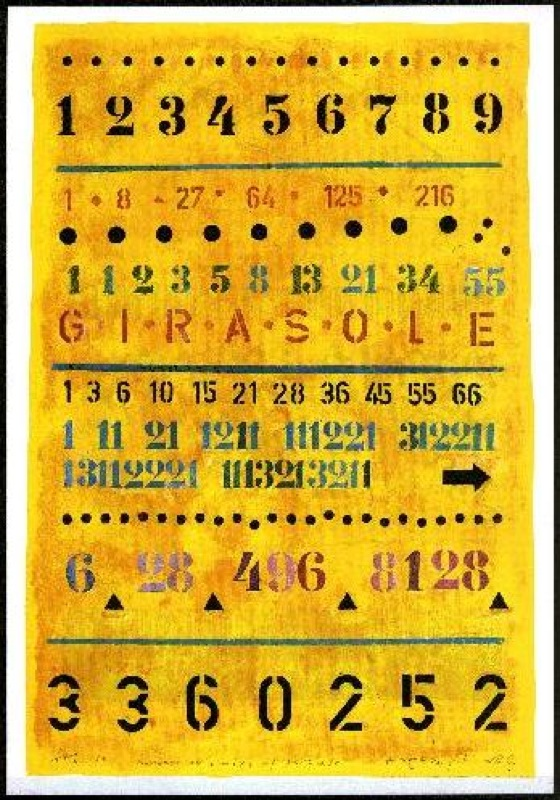
\includegraphics[width=0.618\textwidth]{pictures/ejost}}
\title{Folgen \& Reihen}
\subtitle{Look up the Number!}
\author{}
\date{}
%\lowertitleback{
%\includegraphics[height=1.1cm]{/Users/jormawassmer/Pictures/logokoeniz.jpg}%
%\copyright Jorma Wassmer
%1. Auflage, Februar 2011
%}


\begin{document}
\maketitle
\tableofcontents
%\thispagestyle{empty}
\cleardoublepage
%\setcounter{page}{1}

\section{Folgen}

\subsection{Basics}
\begin{wrapfigure}{r}{0.382\textwidth}
\vspace{-2pt}
  \begin{center}
    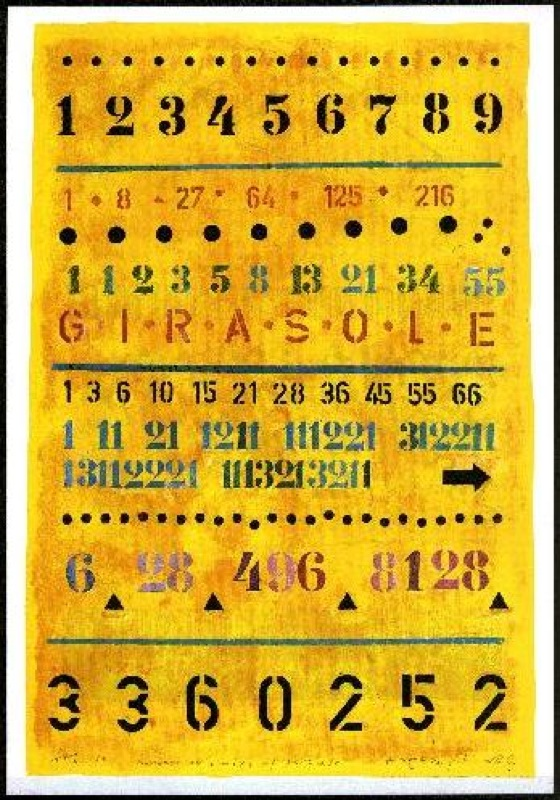
\includegraphics[width=0.33\textwidth]{pictures/ejost}
  \end{center}
\caption{You Know my Name}
\vspace{-30pt}
\end{wrapfigure}
Das Bild \glqq You know my name (Look up the number)\grqq\ ist vom Thuner K\"unstler \textsc{Eugen Jost}. Suche Gesetzm\"assigkeiten in den Zahlenfolgen.
Beschreibe gefundene Gesetzm\"assigkeiten in Worten und mathematisch. Wie lautet die hundertste Zahl der jeweiligen Folge? Wie lautet die $k$-te Zahl der Folge?

\begin{ueb}[Papier falten]
Man falte einen Bogen Papier in der Mitte und lege die beiden H\"alften aufeinander. Danach setze man dieses Prozedere mit dem gefalteten Papier fort.
\begin{enumeratea}
\item Wie oft kann man das Papier h\"och\-stens falten?
\item Man denkt sich nach jeder Faltung das Papier l\"angs der Falt\-achse aufgeschnitten und die beiden H\"alf\-ten zu einem Turm aufgeschichtet. Wie hoch ist der Turm nach $2,3,4,5$ Faltungen?
\item Finde den Zusammenhang zwischen der Turm\-h\"ohe $h_k$ und der Anzahl Faltungen $k\in\mN$.
\item Wie hoch ist der Turm nach $15,20,42$ Faltungen? Sch\"at\-ze zuerst.
\end{enumeratea}
\end{ueb}

\begin{bem}
Man ahnt aus obiger Übung den Zusammenhang zwischen dieser \glqq Art\grqq\ von Folge und Exponentialfunktion. Hier ist der Unterschied zu einer Exponentialfunktion bloss, dass man nur an diskreten Werten --- bzw. ihren Funktionswerten --- interessiert ist.
\end{bem}
Eine Zahlenfolge ist eine Folge, die nur aus Zahlen besteht. Die einzelnen Zahlen der Folge nennt man Glieder. Es ist naheliegend, jedem Glied einer bestimmten Folge seine Positionsnummer zuzuordnen.
Um Unklarheiten aus dem Weg zu r\"aumen und den Begriff der Folge global zu erfassen, definieren wir unmissverst\"andlich, was wir unter einer Folge verstehen wollen.
\begin{cdef}[Folge]{Folge}
Eine \textbf{Folge} ist eine Funktion
$$f:\mD\longrightarrow\mW,$$
deren Definitionsmenge die Menge der nat\"urlichen Zahlen, oder eine Teilmenge davon, ist.
\end{cdef}
Besteht die Folge aus lauter reellen Zahlen, so spricht man genauer von einer Zahlenfolge.
\begin{cdef}[Zahlenfolge]{}
Eine \textbf{Zahlenfolge} ist eine Funktion
$$f:\D{D}\longrightarrow\D{R}$$
mit $\D{D}\subset\D{N}$.
\end{cdef}
\begin{bem}
H\"aufig wird die Bemerkung $k\in\D{N}$ weggelassen, weil sie aus dem Kontext hervorgeht. Betrachtet man Folgen, die nicht unendlich lang sind, dann sollte man die Defi\-ni\-tions\-menge explizite angeben.
\end{bem}
\begin{cdef}[Glied der Folge]{}
Die reellen Zahlen
$$a_1\q a_2\q a_3\q\dots\q a_{k-1}\q a_k\q a_{k+1}\q\dots$$
einer Zahlenfolge heissen Glieder der Folge. $a_k$, die kurze Schreibweise von $f(k)$, heisst $k$-tes \textbf{Glied} der Folge.
\end{cdef}
\begin{bem}
Der Index $k$ kann also als Position in der jeweiligen Folge aufgefasst werden. $a_k$ hingegen ist der Wert, der an Position $k$ steht.
\end{bem}
\begin{bsps}
Zur Illustration einige Beispiele:
\begin{itemize}
\item $a_k=2k$ ist die Folge der geraden Zahlen
$$2\q4\q6\q8\q\dots,$$
denn es ist $a_1=2$, $a_2=4$, $a_3=6$, etc.
\item $a_k=2k-1$
$$1\q3\q5\q7\q\dots$$
\item $a_k=k^2$
$$1\q4\q9\q16\q\dots$$
\end{itemize}
\end{bsps}
\begin{ueb}[Schreibweise]
Notiere die ersten f\"unf Glieder der Folgen aus obigem Beispiel und beschreibe sie in Worten.
\end{ueb}
Die Definition einer Folge l\"asst nat\"urlich auch solche zu, die keinen Gesetzm\"assigkeiten folgen und zu denen man daher jedes Glied explizite angeben muss. Wir werden uns hier aber haupts\"achlich mit speziell einfach zu beschreibenden Folgen befassen.
\begin{ueb}[Einsetz\"ubung]
Berechne die ersten sechs, das hundertste und das $101$-ste Glied der Folge:

\begin{minipage}{0.3\textwidth}
\begin{enumeratea}
\item $a_k=3k-5$
\item $b_k=\frac{k}{k+1}$
\end{enumeratea}
\end{minipage}
\begin{minipage}{0.3\textwidth}
\begin{enumeratea}
\addtocounter{enumi}{2}
\item $c_k=\left(1+\frac{1}{k}\right)^k$
\item $d_k=\sin\left(\frac{k\pi}{2}\right)$
\end{enumeratea}
\end{minipage}
\end{ueb}

\begin{ueb}[Muster erkennen]
Ermittle das $k$-te Glied der Folge:

\begin{minipage}{0.3\textwidth}
\begin{enumeratea}
\item $3,8,13,18,23,\dots$
\item $1,3,7,15,31,\dots$
\end{enumeratea}
\end{minipage}
\begin{minipage}{0.3\textwidth}
\begin{enumeratea}
\addtocounter{enumi}{2}
\item $-1,4,-9,16,-25,\dots$
\item $2,6,12,20,30,\dots$
\end{enumeratea}
\end{minipage}
\end{ueb}

\begin{bem}
Bei vielen Zahlenfolgen ist es schwierig, die Vorschrift zu finden, mit der man das $k$-te Glied direkt berechnen kann. Jedoch kann man oft ein Bildungsgesetz erkennen, das f\"ur jede nat\"urliche Zahl $k$ die Berechnung von $a_k$ aus $a_{k-1}$ erm\"oglicht, d.h. die Berechnung des Wertes an Position $k$ anhand des Wertes der vorherigen Position.
\end{bem}

\subsection{Explizite und rekursive Beschreibungen von Folgen}
Explizite und rekursive Definitionen von Folgen sind zwei M\"oglichkeiten, Folgen zu beschreiben.

Bei der \textbf{expliziten Definition} einer Folge erh\"alt man ein beliebiges Glied sofort aus der Funktionsvorschrift, indem man direkt einsetzt. Beispielsweise ist $a_k=2k$ eine explizite Definition der Folge der geraden Zahlen.

\begin{bsp}
Eine explizite Definition von $1,3,7,15,31,\dots$
ist
$$a_k=2^k-1.$$
\end{bsp}

Bei der \textbf{rekursiven Definition} einer Folge ergibt sich das $k$-te Glied aus den vorherigen Gliedern mit Hilfe einer sogenannten Rekursionsvorschrift. Bei dieser Definition m\"ussen dann auch so viele Glieder explizite vorgegeben werden, wie die Rekursionsvorschrift \glqq zum Starten\grqq\ ben\"otigt.

\begin{bsp}
Eine Rekursionsformel f\"ur $1,3,7,15,31,\dots$
ist
$$a_k=2\cdot a_{k-1}+1,\q a_1=1.$$
\end{bsp}

\begin{bsp}
Die \textbf{Fibonacci-Folge}
$$1\q1\q2\q3\q5\q8\q13\q21\q\dots$$
kann durch
$$a_k=a_{k-1}+a_{k-2}\q\text{mit }a_1=1\text{ und }a_2=1$$
rekursiv definiert werden.
\end{bsp}

\begin{bem}
Die Fibonacci-Folge ist \"ausserst ber\"uhmt. Benannt ist sie nach \textsc{Leonardo Fibonacci}, der damit im Jahr $1202$ das Wachstum einer Kaninchenpopulation beschrieb. Die Folge war aber schon in der Antike sowohl den Griechen als auch den Indern bekannt. Sie wird heute oft von K\"unstlern benutzt und in Film, Musik, Bildern u.\"a. verk\"orpert.
\end{bem}

\begin{bem}
F\"ur viele Zahlenfolgen k\"onnen sowohl rekursive als auch explizite Definitionen gefunden werden. Zum Beispiel ist
$$a_k=\frac{1}{\sqrt{5}}\left(\frac{1+\sqrt{5}}{2}\right)^k - \frac{1}{\sqrt{5}}\left(\frac{1-\sqrt{5}}{2}\right)^k$$
eine explizite Definition der Fibonacci-Folge, die von \textsc{de Moivre} 1718 hergeleitet wurde.. Teste sie!
\end{bem}

\begin{ueb}[Muster erkennen 2]
Finde ein Bildungsgesetzt f\"ur die Folge; falls m\"oglich explizit. Beschreibe notfalls ein Bildungsverfahren.

\begin{minipage}{0.4\textwidth}
\begin{enumeratea}
\item $1,8,27,64,125,\dots$
\item $1,2,6,24,120,\dots$
\end{enumeratea}
\end{minipage}
\begin{minipage}{0.4\textwidth}
\begin{enumeratea}
\setcounter{enumi}{2}
\item $2,3,5,7,11,\dots$
\item $0,1,0,-1,0,1,\dots$
\end{enumeratea}
\end{minipage}
\end{ueb}

\begin{ueb}[rekursiv formulieren]
Gib eine m\"ogliche rekursive Definition f\"ur die Folge
\begin{enumeratea}
\item $-7,-3,1,5,9,\dots$
\item $10,12,15,19,24,30,\dots$
\item $c_k=k\cdot2^k$
\item die Innenwinkelsumme eines $n$-Ecks $w_n$
\item die maximale Anzahl der Schnittpunkt von $n$ Geraden $s_n$
\end{enumeratea}
\end{ueb}

\subsection{Die Partialsumme einer Folge}
H\"aufig ist an einer Zahlenfolge interessant, wie gross nun die Summe ihrer Glieder ist.
Hat man also eine Zahlenfolge
$$a_1\q a_2 \q\, a_3\q \dots$$
so lautet die zugeh\"orige Summe bis zum $n$-ten Glied
$$a_1+a_2+a_3+\dots+a_n.$$

Deshalb definiert man:
\pagebreak
\begin{cdef}[Partialsumme]{}
Die
\marginnote{
\qrcode{
https://www.youtube.com/watch?v=G_PSp59zNJc}
}
$k$-te \textbf{Partialsumme} der ersten $k$ oder aller Glieder einer Zahlenfolge ist die Summe
$$s_n=a_1+a_2+\ldots+a_{k-1}+a_k$$
\end{cdef}

\begin{ueb}[Summen bilden]
Berechne die erste, dritte, 100., $n$-te Partialsumme der Folge
$$1\q2\q3\q4\q\dots$$
Tipp: Verwende Kombinatorik oder den Trick von C.F.~Gauss.
\end{ueb}

\begin{bem}
Man schreibt eine Summe --- oder Reihe --- wie folgt etwas k\"urzer:
$$a_1+a_2+a_3+\dots+a_n = \sum_{k=1}^{n}a_k.$$
Dabei schreibt man also ein grosses $\Sigma$ (Sigma), um anzudeuten, dass es sich um eine Summe handelt. Unterhalb dieses Sigmas wird notiert, bei welchem nat\"urlichen Wert die laufende Variable (hier $k$) startet. Dieses $k$ wird solange um $1$ erh\"oht, bis es die obere Grenze $n$ erreicht hat. Zwischen den Erh\"ohungen wird immer ein $+$-Zeichen gesetzt.
\end{bem}
\begin{bsps}
\begin{align}
\notag
\sum_{k=1}^{n}k &=1+2+3+4+\dots +n\\ \notag
\sum_{k=1}^{n}k^2 &=1^2+2^2+3^2+4^2+\dots+n^2\\ \notag
\sum_{k=100}^{999}k &=100+101+102+\dots+999
\end{align}
\end{bsps}
\begin{bem}

Man kann aus einer Zahlenfolge eine neue zusammenstellen, welche einfach aus den verschiedenen Teilsummen der urspr\"unglichen Zahlenfolge besteht. Wenn man beispielsweise die Zahlenfolge
$$1\q2\q3\q4\q5\dots$$
anschaut, dann ist ihre erste Teilsumme $s_1=1$, ihre zweite $s_2=3$, die dritte $s_3=6$, die vierte $s_4=10$, etc. Man kann also eine Folge der Teilsummen
$$1\q3\q6\q10\q15\q21\dots$$
bestehend aus den einzelnen Teilsummen
$$s_k=\sum_{i=1}^{k}i$$
bilden.
\end{bem}

\begin{ueb}[Folgeprodukt]
Stelle folgenden Ausdruck mit einem einzigen Term dar
$$s_k=\frac{1}{1\cdot2}+\frac{1}{2\cdot3}+\frac{1}{3\cdot4}+\frac{1}{4\cdot5}+\dots+\frac{1}{k\cdot(k+1)}$$
Berechne dazu erst einmal die Summe der ersten paar Glieder, also $s_1, s_2, s_3,\dots$, explizite, und versuche dann eine Formel f\"ur obigen Ausdruck zu erraten, die den Wert von $s_k$ explizite angibt.
\end{ueb}

\begin{ueb}[Zweierpotenzen-Kehrwert]
Wie vorhergehende Übung, aber mit dem Ausdruck
$$s_k=1+\frac{1}{2}+\frac{1}{4}+\frac{1}{8}+\dots+a_k$$
Finde zuerst eine Darstellung f\"ur $a_k$.
\end{ueb}

Im Folgenden werden wir uns fast ausschliesslich auf zwei Typen von Zahlenfolgen beschr\"anken. N\"amlich einerseits auf Folgen, bei denen der \glqq Abstand\grqq\ zweier aufeinander folgender Glieder konstant ist (verwandt mit affinen Funktionen), und andererseits auf Folgen, bei denen der Quotient zweier aufeinander folgender Glieder konstant ist (verwandt mit Exponentialfuntionen).

\section{Arithmetische Folgen \&\ Reihen}

\begin{cdef}[Arithmetische Folge]{}
Eine
\marginnote{
\qrcode{
https://www.youtube.com/watch?v=zGVcjrRe1Hg}
}
\textbf{arithmetische Folge} ist eine Zahlenfolge, deren Glieder der Rekursionsformel
$$a_{k+1}=a_k+d\q (k\in\mN, d=\text{konstant})$$
gen\"ugen.
\end{cdef}

\begin{bem}
Der Name arithmetische Folge ist dadurch motiviert, dass jedes Glied --- ausser das erste und gegebenenfalls das letzte --- gleich dem arithmetischen Mittel der Nachbarglieder ist.
\end{bem}

\begin{ueb}[Name \glqq arithmetisch\grqq]
Zeige die G\"ultigkeit der obigen Bemerkung.
\end{ueb}

\begin{bsp}
Die Folge der ungeraden nat\"urlichen Zahlen ist arithmetisch mit $d=2$.
$$1\q3\q5\q7\q9\q\dots$$
\end{bsp}

\pagebreak

\begin{csatz}[AF Formeln]{}\label{arithformeln}
F\"ur eine arithmetische Folge gelten
\begin{align}
a_k&=a_1+(k-1)\cdot d\label{arithglied}\\
s_k&=k\cdot\frac{a_1+a_k}{2}\label{arithsum}
\end{align}
\end{csatz}

\begin{proof}[Beweis]
(\ref{arithglied}) ist eine \glqq Pf\"ostchen-†berlegung\grqq. F\"ur (\ref{arithsum}) nimmt man den Trick von Gauss.
\end{proof}

\begin{ueb}[Dreierzahlen]
Berechne die Summe aller Dreierzahlen von $81$ bis $1020$.
\end{ueb}

\begin{ueb}[freier Fall]
Ein frei fallender K\"orper legt in der ersten Sekunde $\unit[5]{m}$ und in jeder folgenden Sekunde $\unit[10]{m}$ mehr als in der jeweils vorangegangenen Sekunde zur\"uck.
\begin{enumeratea}
\item Welche Strecke legt er in der 13-ten Sekunde zur\"uck?
\item Welche Strecke f\"allt er in $\unit[13]{Sekunden}$?
\item Wie viele Sekunden braucht er f\"ur $\unit[1805]{m}$?
\end{enumeratea}
\end{ueb}

\section{Geometrische Folgen \&\ Reihen}

\begin{cdef}[geometrische Folge]{}
Eine
\marginnote{
\qrcode{
https://www.youtube.com/watch?v=b0rjVBStXGo}
}
\textbf{geometrische Folge} ist eine Zahlenfolge, deren Glieder der Rekursionsformel
$$a_{k+1}=a_k\cdot q\q(k\in\mN, q=\text{konstant})$$
gen\"ugen.
\end{cdef}

\begin{bem}
Der Name geometrische Folge ist dadurch motiviert, dass jedes Glied --- ausser das erste und gegebenenfalls das letzte --- gleich dem geometrischen Mittel der Betr\"age Nachbarglieder ist.
\end{bem}

\begin{ueb}[Name geometrisch]
Zeige die G\"ultigkeit der obigen Bemerkung.
\end{ueb}

\begin{bsp}
Die Folge der Zweierpotenzen mit nat\"urlichen Exponenten ist geometrisch mit $q=2$.
$$2\q4\q8\q16\q32\q\dots$$
\end{bsp}

\pagebreak

\begin{csatz}[GF Formeln]{}\label{geomformeln}
F\"ur eine geometrische Folge gelten
\begin{align}
a_k&=a_1\cdot q^{k-1}\label{geomglied}\\
s_k&=a_1\cdot\frac{q^k-1}{q-1}\label{geomsum}
\end{align}
\end{csatz}

\begin{proof}[Beweis]
(\ref{geomglied}) ist wiederum eine \glqq Pf\"ostchen-\"Uberlegung\grqq. Wir zeigen (\ref{geomsum}) und nehmen dazu an, dass die Folge endlich sei.
\begin{align*}
s_k&=a_1+a_2+a_3+\ldots+a_k\\
&=a_1+a_1\cdot q+a_1\cdot q^2+\ldots+a_1\cdot q^{k-1}
\end{align*}
Multipliziert man diese Gleichung mit $q$ folgt
$$s_k\cdot q=a_1\cdot q+a_1\cdot q^2+a_1\cdot q^3+\ldots+a_1\cdot q^k$$
Nun subtrahieren wir $s_k$ von $s_k\cdot q$ und erhalten
$$s_k\cdot q-s_k=s_k(q-1)=a_1\cdot q^k-a_1=a_1(q^k-1)$$
Daraus folgt unmittelbar
$$s_k=\frac{a_1(q^k-1)}{q-1}$$
und damit die Behauptung.
\end{proof}

\begin{ueb}[Zweierpotenzen]
Berechne
$$-2+4-8+16-\dots+4096.$$
\end{ueb}

\begin{ueb}[Zwischen 1 und 2]
Eine geometrische Folge besteht aus 10 positiven Gliedern, beginnt mit $1$ und endet mit $2$. Bestimme das Bildungsgesetz dieser Folge und berechne die zugeh\"orige Partialsumme aller Glieder.
\end{ueb}

\section{\"Ubungen zu arithmetischen und geometrischen Folgen}

\begin{ueb}[Rohr-Pyramide]
Es sind 60 Rohre so zu stapeln, dass jede Schicht auf L\"ucke mit der darunter liegenden Schicht liegt; die oberste Schicht soll aus vier Rohren bestehen. Wie viele Rohre m\"ussen in die unterste Schicht gelegt werden, und wie viele Schichten hat der Stapel? Wie hoch ist er, wenn die Rohre einen Durchmesser von $\unit[20]{cm}$ haben?
\end{ueb}

\begin{ueb}[Kalium]
F\"ur manche medizinische Diagnosen wird das radioaktive Kaliumisotop $^{42}$K benutzt. Es verliert pro Stunde $5.42\%$ seiner Intensit\"at. Welchen Prozentsatz verliert es nach drei Stunden?
\end{ueb}

\begin{ueb}[AF und GF]
$a, b, c$ bilden in dieser Reihenfolge eine arithmetische Folge mit der Summe $3$; in der Reihenfolge $b, c, a$ bilden sie eine geometrische Folge. Berechne die drei Zahlen, wenn $a\neq b\neq c$.
\end{ueb}

\begin{ueb}[Reisk\"orner]
In
\marginnote{
\qrcode{
https://www.youtube.com/watch?v=UGOdwBEIbWc}
}
einer Erz\"ahlung des Persers \textsc{Ibn Khallikan} aus dem 13.Jahrhundert lesen wir: \glqq In jener Zeit, als der indische Herrscher \textsc{Shihram} seine Untertanen unm\"assig tyrannisierte, erfand der Weise \textsc{Sissa Ibn Dahir} zur Belehrung des K\"onigs das Schachspiel, um ihm nachzuweisen, wie wichtig f\"ur einen Herrscher seine Untertanen sind. Als Dank f\"ur die Erleuchtung bot der K\"onig \textsc{Sissa} seine Sch\"atze an und stellte ihm einen Wunsch frei. Der Weise w\"unschte sich soviel Weizen, wie sich auf dem Schachbrett folgendermassen angeordnet ergibt: Auf das erste Feld des Schachbrettes 1 Reiskorn, auf das zweite Feld 2 Reisk\"orner, auf das dritte Feld 4 K\"orner etc., auf jedem Feld doppelt so viele wie auf dem vorhergehenden.\grqq
\begin{enumeratea}
\item Wie viele Reisk\"orner sind dies insgesamt?
\item Wie lange w\"are ein Zug, der diese Reismenge transportieren m\"usste, wenn ein G\"uterwagen von $\unit[10]{m}$ L\"ange $\unit[10]{Tonnen}$ Reis laden kann und  $18$ K\"orner $\unit[1]{g}$ ergeben?
\item Welche H\"ohe h\"atte ein Reisteppich, wenn man die Schweiz damit bedecken w\"urde? (Nimm z.B. ein zylindrisches Reiskorn mit Durchmesser $\unit[2]{mm}$ und H\"ohe $\unit[1]{cm}$.)
\end{enumeratea}
\end{ueb}

\begin{ueb}[Quadrate]
Die Figuren sind aus Quadraten zusammengesetzt wie in Abbildung \ref{ueb:quadrate} auf Seite \pageref{ueb:quadrate}.
\begin{figure}
\centering
\definecolor{zzttqq}{rgb}{0.6,0.2,0}
\definecolor{cqcqcq}{rgb}{0.75,0.75,0.75}
\scalebox{1.2}{
\begin{tikzpicture}[line cap=round,line join=round,>=triangle 45,x=0.45cm,y=0.45cm]
\draw [color=cqcqcq,dash pattern=on 2pt off 2pt, xstep=0.45cm,ystep=0.45cm] (-2.6,-1.28) grid (11.6,6.3);
\clip(-2.6,-1.28) rectangle (11.6,6.3);
\fill[line width=1.6pt,color=zzttqq,fill=zzttqq,fill opacity=0.15] (-2,2) -- (-1,2) -- (-1,3) -- (-2,3) -- cycle;
\fill[line width=1.6pt,color=zzttqq,fill=zzttqq,fill opacity=0.15] (2,3) -- (2,4) -- (3,4) -- (3,3) -- (4,3) -- (4,2) -- (3,2) -- (3,1) -- (2,1) -- (2,2) -- (1,2) -- (1,3) -- cycle;
\fill[line width=1.6pt,color=zzttqq,fill=zzttqq,fill opacity=0.15] (6,3) -- (7,3) -- (7,4) -- (8,4) -- (8,5) -- (9,5) -- (9,4) -- (10,4) -- (10,3) -- (11,3) -- (11,2) -- (10,2) -- (10,1) -- (9,1) -- (9,0) -- (8,0) -- (8,1) -- (7,1) -- (7,2) -- (6,2) -- cycle;
\draw [line width=1.6pt,color=zzttqq] (-2,2)-- (-1,2);
\draw [line width=1.6pt,color=zzttqq] (-1,2)-- (-1,3);
\draw [line width=1.6pt,color=zzttqq] (-1,3)-- (-2,3);
\draw [line width=1.6pt,color=zzttqq] (-2,3)-- (-2,2);
\draw [line width=1.6pt,color=zzttqq] (2,3)-- (2,4);
\draw [line width=1.6pt,color=zzttqq] (2,4)-- (3,4);
\draw [line width=1.6pt,color=zzttqq] (3,4)-- (3,3);
\draw [line width=1.6pt,color=zzttqq] (3,3)-- (4,3);
\draw [line width=1.6pt,color=zzttqq] (4,3)-- (4,2);
\draw [line width=1.6pt,color=zzttqq] (4,2)-- (3,2);
\draw [line width=1.6pt,color=zzttqq] (3,2)-- (3,1);
\draw [line width=1.6pt,color=zzttqq] (3,1)-- (2,1);
\draw [line width=1.6pt,color=zzttqq] (2,1)-- (2,2);
\draw [line width=1.6pt,color=zzttqq] (2,2)-- (1,2);
\draw [line width=1.6pt,color=zzttqq] (1,2)-- (1,3);
\draw [line width=1.6pt,color=zzttqq] (1,3)-- (2,3);
\draw [line width=1.6pt,color=zzttqq] (6,3)-- (7,3);
\draw [line width=1.6pt,color=zzttqq] (7,3)-- (7,4);
\draw [line width=1.6pt,color=zzttqq] (7,4)-- (8,4);
\draw [line width=1.6pt,color=zzttqq] (8,4)-- (8,5);
\draw [line width=1.6pt,color=zzttqq] (8,5)-- (9,5);
\draw [line width=1.6pt,color=zzttqq] (9,5)-- (9,4);
\draw [line width=1.6pt,color=zzttqq] (9,4)-- (10,4);
\draw [line width=1.6pt,color=zzttqq] (10,4)-- (10,3);
\draw [line width=1.6pt,color=zzttqq] (10,3)-- (11,3);
\draw [line width=1.6pt,color=zzttqq] (11,3)-- (11,2);
\draw [line width=1.6pt,color=zzttqq] (11,2)-- (10,2);
\draw [line width=1.6pt,color=zzttqq] (10,2)-- (10,1);
\draw [line width=1.6pt,color=zzttqq] (10,1)-- (9,1);
\draw [line width=1.6pt,color=zzttqq] (9,1)-- (9,0);
\draw [line width=1.6pt,color=zzttqq] (9,0)-- (8,0);
\draw [line width=1.6pt,color=zzttqq] (8,0)-- (8,1);
\draw [line width=1.6pt,color=zzttqq] (8,1)-- (7,1);
\draw [line width=1.6pt,color=zzttqq] (7,1)-- (7,2);
\draw [line width=1.6pt,color=zzttqq] (7,2)-- (6,2);
\draw [line width=1.6pt,color=zzttqq] (6,2)-- (6,3);
\end{tikzpicture}
}
\caption{Quadrate}\label{ueb:quadrate}
\end{figure}
Stelle eine Formel auf f\"ur die Anzahl $A(k)$ der Quadrate, die in der $n$-ten Figur vorhanden sind.
\end{ueb}

\begin{ueb}
In
\marginnote{
\qrcode{
https://www.youtube.com/watch?v=AJtWxcZNq28}
}
der Randnotiz findet man ein Video zur Matura Mathematik Aufgabe Folgen und Reihen von 2013. Darin seht ihr die Aufgabe und eine mögliche Lösung kommentiert.
\end{ueb}

\section{Grenzwerte}
\subsection{Konvergenz und bestimmte Divergenz}
\begin{wrapfigure}{r}{0.382\textwidth}
\vspace{-23pt}
  \begin{center}
    
\includegraphics[width=0.36\textwidth]{pictures/limit}
  \end{center}
%\caption{A gull}
\vspace{-20pt}
\end{wrapfigure}
Bisher haben wir nur die Anfangsglieder einer Folge betrachtet. Wir wenden uns in diesem Kapitel den Gliedern mit hohen Nummern zu und werden versuchen, Aussagen \"uber ihr Verhalten zu machen, wenn $n$ gegen Unendlich strebt (schreibe: $n\to\infty$).
Wir schreiben f\"ur eine Zahlenfolge $f:\mN\to\mR, k\mapsto f(k)$ kurz $<a_k>$.

\begin{ueb}[konvergent \&\ bestimmt divergent, oder sonst was]
Berechne f\"ur $k=10,11,10^3,10^3+1,10^6,10^6+1$ die Glieder der Zahlenfolge mit

\begin{minipage}{0.3\textwidth}
\begin{enumeratea}
\item $a_k=5+\frac{1}{k}$
\item $b_k=(-1)^k\cdot\frac{3000}{k}$
\end{enumeratea}
\end{minipage}
\begin{minipage}{3.9cm}
\begin{enumeratea}
\addtocounter{enumi}{2}
\item $c_k=k^3$
\item $d_k=1+(-1)^k$
\end{enumeratea}
\end{minipage}
\end{ueb}

Wir k\"onnen also das Verhalten von Folgen f\"ur grosse $k\in\mN$ in drei wesentliche F\"alle aufteilen.
\begin{itemize}
\item[A] Die Glieder der Folge streben f\"ur $k\to\infty$ genau einer reellen Zahl, einem Grenzwert, zu.
\item[B] Die Glieder der Folge werden f\"ur $k\to\infty$ betragsm\"assig gr\"osser als jede noch so grosse Zahl.
\item[C] Die Glieder der Folge verhalten sich nicht so wie in den beiden andern F\"allen.
\end{itemize}
Im Fall A nennt man die Folge konvergent, im Fall B bestimmt divergent.

\subsection{Der Konvergenzbegriff}

Um den Begriff der Konvergenz exakter bereitzustellen betrachten wir ein Beispiel. F\"ur diesen, etwas l\"anger dauernden, Prozess brauchen wir vorerst

\begin{cdef}[Umgebung]{}
Sei $\ge>0$ eine positive reelle Zahl und $g\in\mR$ beliebig. Das offene Intervall $(g-\ge,g+\ge)$ heisst \textbf{$\ge$-Umgebung} von $g$.
\end{cdef}

\begin{bsp}
Wir betrachten die Zahlenfolge
$$a_k=2+(-1)^k\cdot\frac{4}{k}$$
und berechnen die ersten sechs Glieder der Folge. Dazu zeichnen wir die $\ge$-Umgebung $1$ um  den Grenzwert $g$, d.h. $g=2$ und $\ge=1$.

\begin{figure}[h!]
\centering
\definecolor{uququq}{rgb}{0.25,0.25,0.25}
\scalebox{1.2}{
\begin{tikzpicture}[line cap=round,line join=round,>=triangle 45,x=0.6cm,y=0.6cm]
\draw[->,color=black] (-1.78,0) -- (9.08,0);
\foreach \x in {1,2,3,4,5,6,7,8}
\draw[shift={(\x,0)},color=black] (0pt,2pt) -- (0pt,-2pt);
\draw[color=black] (8.74,0.08) node [anchor=south west] { $k$};
\draw[->,color=black] (0,-2.48) -- (0,4.66);
\foreach \y in {-2,-1,1,2,3,4}
\draw[shift={(0,\y)},color=black] (2pt,0pt) -- (-2pt,0pt);
\draw[color=black] (0.1,4.26) node [anchor=west] { $a_k$};
\clip(-1.78,-2.48) rectangle (9.08,4.66);
\draw (-0.8,2.5) node[anchor=north west] {$2$};
\draw (-1.7,3.5) node[anchor=north west] {$2+\epsilon$};
\draw (-1.7,1.5) node[anchor=north west] {$2-\epsilon$};
\draw[dash pattern=on 3pt off 3pt, smooth,samples=100,domain=0.0:9.08] plot(\x,{3});
\draw[dash pattern=on 3pt off 3pt, smooth,samples=100,domain=0.0:9.08] plot(\x,{1});
\draw (0.65,-0.1) node[anchor=north west] {$1$};
\draw (3.65,-0.1) node[anchor=north west] {$N$};
\draw (4.65,-0.1) node[anchor=north west] {$5$};
\draw[color=black] (9.24,1.4) node {$f$};
\fill [color=uququq] (2,4) circle (1.5pt);
\fill [color=uququq] (1,-2) circle (1.5pt);
\fill [color=uququq] (3,0.67) circle (1.5pt);
\fill [color=uququq] (4,3) circle (1.5pt);
\fill [color=uququq] (5,1.2) circle (1.5pt);
\fill [color=uququq] (6,2.67) circle (1.5pt);
\fill [color=uququq] (7,1.43) circle (1.5pt);
\fill [color=uququq] (8,2.5) circle (1.5pt);
\end{tikzpicture}
}
\caption{Veranschaulichung der $\ge$-Um\-ge\-bung}
\end{figure}

Je gr\"osser die Nummern der Glieder gew\"ahlt werden, desto n\"aher sind diese beim Wert $2$. In diesem Beispiel sieht man, dass alle Glieder ab der Nummer $N=4$ in unserer gew\"ahlten Umgebung liegen.
$$\abs{a_k-2}<1\q\text{f\"ur }k>4.$$
W\"ahlt man statt $\ge=1$ nun ein kleineres $\ge$, so kann man bei dieser Folge wieder eine bestimmte Nummer $N$ finden, ab welcher $a_k$ mit $k>N$ in dieser neuen $\ge$-Umgebung liegen. Weil also dieses $N$ von der Gr\"osse der Umgebung abh\"angt, schreibt man oft deutlicher $N(\ge)$ und nennt diese Nummer \textbf{Stichzahl}.
\end{bsp}

\begin{ueb}[Stichzahl]
Berechne zu obiger Folge die Stichzahl $N(\frac{1}{100})$ f\"ur den Grenzwert $g=2$, den wir ja zu kennen glauben.
\end{ueb}

Damit ist $N(0.01) = 400$. Vom $401.$ Glied an liegen alle
Glieder der Folge in der $\frac{1}{100}$-Umgebung von 2. Entsprechend gilt f\"ur alle Glieder mit den Nummern $k > 4000000$: $\abs{a_k - 2} < 0.000001$. Durch passende Wahl einer Gliednummer $N$ kann man bei dieser Folge immer erreichen, dass von dieser Nummer an alle Betragsdifferenzen $\abs{a_k - 2}$ kleiner als jede noch so klein gew\"ahlte Zahl $\ge$ ausfallen. Man sagt dann, dass
die Folge $<a_k>$ konvergiert und den
Grenzwert $g=2$ hat.

\begin{cdef}[Konvergenz]{}
Eine
\marginnote{
\qrcode{
https://www.youtube.com/watch?v=yarhoKJglDo}
}
Folge $<a_k>$ heisst \textbf{konvergent mit Grenzwert $g$}, wenn zu jeder noch so kleinen $\ge$-Umgebung von $g$ eine Nummer $N(\ge)$ so existiert, dass alle Glieder $a_k$ mit $k > N(\ge)$ in dieser Umgebung liegen. Kurz:
$$\forall\ge>0\q\exists N(\ge)\text{ so, dass }\abs{a_k-g}<\ge\q\forall k>N(\ge)$$
\end{cdef}

\begin{bem}
Ausschlaggebend f\"ur die Konvergenz einer Folge ist die Existenz von $N$; v\"ollig belanglos ist die Gr\"osse.
\end{bem}

\begin{bem}
Konvergiert die Folge $<a_k>$ gegen den Grenzwert $g$ (Fall A), so schreibt man daf\"ur
$$\lim_{k\to\infty}a_k=g$$
F\"ur die bestimmt divergenten Folgen, deren Glieder gegen $\infty$ oder gegen $-\infty$ streben (Fall B), benutzt man die gleiche Symbolik und schreibt:
$$\lim_{k\to\infty}a_k=\infty\q\text { bzw. }\q\lim_{k\to\infty}a_k=-\infty$$
\end{bem}
Das Symbol $\infty$ stammt von \textsc{John Wallis} (1616-1703), der Begriff \glqq limes\grqq\ (lat. Grenze) von \textsc{Isaak Newton} (1643-1716) und die Bezeichnung \glqq Konvergenz\grqq\ von \textsc{James Gregory} (1638-1675).

\begin{ueb}[Umgebung]
Untersuche die Folge mit

\begin{minipage}{0.3\textwidth}
\begin{enumeratea}
\item $a_k=\frac{5}{k+1}$
\item $b_k=\frac{7k+8}{2k-3}$
\end{enumeratea}
\end{minipage}
\begin{minipage}{0.4\textwidth}
\begin{enumeratea}
\setcounter{enumi}{2}
\item $x_k=k^2-3$
\item $u_k=\frac{3-2k^2}{k^2}$
\end{enumeratea}
\end{minipage}

auf Konvergenz. Berechne, falls die Folge konvergent ist, die Nummern $N(10^{-3})$ und $N(\ge)$ f\"ur ein beliebiges $\ge$. Veranschauliche dir mit einer Figur den Sachverhalt.
\end{ueb}

\subsection{Ausblick}
Man kann die Konvergenz einer Folge auch nachweisen, ohne den Grenzwert zu kennen. Das von \textsc{Augustin Louis Cauchy} (1789 - 1857) stammende Konvergenzkriterium besagt n\"amlich, dass eine Folge konvergiert, wenn der Unterschied beliebiger Folgenglieder mit gen\"ugend grosser Nummer kleiner als jede vorgegebene positive reelle Zahl ist.

\begin{cdef}[monoton]{}
Eine Folge $<a_k>$ heisst \textbf{monoton wachsend}, wenn $a_{k+1}\geq a_k$ resp. \textbf{monoton fallend}, wenn $a_{k+1}\leq a_k$ f\"ur alle $k$ ist.
\end{cdef}

\begin{cdef}[beschränkt]{}
Eine Folge $<a_k>$ heisst \textbf{beschr\"ankt}, wenn es eine positive Zahl $M$ mit $\abs{a_k}< M$ f\"ur alle $k$ gibt.
\end{cdef}

\clearpage

\section{Reihen}
\begin{wrapfigure}{R}{0.382\textwidth}
\vspace{-15pt}
  \begin{center}
    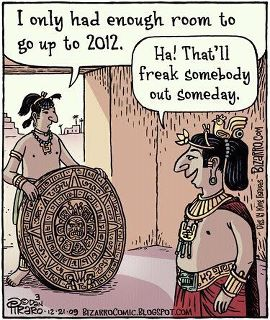
\includegraphics[width=0.37\textwidth]{pictures/2012}
  \end{center}
%\caption{A gull}
\vspace{-60pt}
\end{wrapfigure}
Reihen spielen nicht nur in der reinen Mathematik eine wichtige Rolle, insbesondere in  der Physik und der Technik sind sie unentbehrlich; deshalb der Titel \emph{Folgen und Reihen}. Mit Reihen kann man beispielsweise die Kreiszahl  $\pi$ und die Funktionswerte der trigonometrischen Funktionen n\"aherungsweise berechnen. Unter einer \textbf{Reihe} verstehen wir die \glqq unendliche\grqq\ Summe einer Folge.

\begin{ueb}[N\"aherungen]
Es gelten die folgenden N\"aherungsformeln:
\begin{align*}
\frac{\pi}{4}&\approx1-\frac{1}{3}+\frac{1}{5}-\frac{1}{7}+\frac{1}{9}\\
\cos(x)&\approx1-\frac{x^2}{2!}+\frac{x^4}{4!}-\frac{x^6}{6!}\\
\frac{1}{1+x}&\approx1-x+x^2-x^3\q\abs{x}<1
\end{align*}
Berechne damit $\pi$, $\cos(\frac{\pi}{3})$ und $\frac{1}{1+0.13}$. Um wie viel Prozent weicht die N\"aherung vom tats\"achlichen Wert ab?
\end{ueb}

Je mehr Summanden ber\"ucksichtigt werden, desto genauer werden die N\"aherungswerte. Die Herleitungen der N\"aherungsformeln f\"ur $\pi$ und $\cos(x)$ sind schwierig und geh\"oren nicht zum Programm der nicht-PAM Maturit\"atstypen. Deshalb verzichten wir hier im Grundlagenfach auf sie. Das dritte Beispiel jedoch wird in einer sp\"ateren Aufgabe begr\"undet.

Der M\"onch \textsc{Guido Grandi}, ein Mathematiker der Universit\"at Pisa, kam 1703 in einer seiner Schriften zu dem Ergebnis:
$$1-1+1-1+1-1+1-\dots=\frac{1}{2}.$$
Obwohl er immer zwei aufeinanderfolgende Summanden zusammenfasste, zog er den Schluss:
$$0+0+0+0+0+0+\dots=\frac{1}{2}.$$
Dies war f\"ur ihn ein Beweis daf\"ur, dass Gott die Welt aus dem Nichts hat erschaffen k\"onnen. Das Universalgenie \textsc{Leibniz} stimmte ihm 1713 mit der folgenden †berlegung zwar nicht in der Interpretation, aber in der Sache zu: Bricht man die Summation nach einer geraden Anzahl von Summanden ab, so erh\"alt man als Summe $0$, bricht man sie nach einer ungeraden Anzahl ab, so erh\"alt man als Summe $1$. Nun gibt es aber unendlich viele Summanden, und da wir dem Unendlichen weder den Charakter einer geraden noch einer ungeraden Zahl zuschreiben k\"onnen, kann die Summe weder den Wert $1$ noch den Wert $0$ haben. Die Wahrscheinlichkeitsrechnung lehrt nun, dass man, wenn zwei Werte f\"ur eine Gr\"osse gleichwahrscheinlich sind, ihr arithmetisches Mittel als den wahren Wert nehmen muss. Daher muss man der Summe, wenn man konsequent sein will, den Wert
$$\frac{1+0}{2}=\frac{1}{2}$$
annehmen. Erst viel sp\"ater erkannte man, dass es sich hier um ein typisches Scheinproblem handelt. Man muss erst definieren, was man unter der Summe von unendlich vielen Summanden versteht, denn das Wort \emph{Summe} ist ja bis anhin nur f\"ur endlich viele Summanden erkl\"art.

\begin{cdef}[Reihe]{}
Es sei $a_1,a_2,a_3, \dots$ eine beliebige reelle Zahlenfolge. Die formal gebildete Summe mit unendlich vielen Summanden
$$a_1+a_2+a_3+\dots$$
heisst eine unendliche Summe oder kurz \textbf{Reihe}.
\end{cdef}
Mit den Folgengliedern bildet man eine neue Folge, die Folge der Partialsummen, sie ist rekursiv definiert durch:
$$s_1=a_1, s_n=s_{n-1}+a_n \text{ f\"ur } n\geq2.$$

Erst durch diese Definition wird die Addition von unendlich vielen Summanden sinnvoll, denn die Glieder der Folge der Partialsummen k\"onnen nun einem bestimmten Wert zustreben oder nicht; entsprechend nennt man die unendliche Reihe konvergent oder bestimmt divergent.

\begin{bsps}
\ \\[-4ex]
\begin{itemize}
\item $a_1=0.9, a_2=0.09, a_3=0.009, \dots$, also $s_1 = 0.9, s_2 = 0.99, s_3 = 0.999, \dots$. Die Folgenglieder $s_n$ streben dem Wert $s=1$ zu; die entsprechende unendliche Reihe ist konvergent.
\item $a_1=5, a_2=6, a_3=7, a_4=8, \dots$, also $s_1 = 5, s_2 = 11, s_3 = 18, s_4 = 26, \dots$. Die Folgenglieder $s_n$ streben keinem bestimmten Wert zu; die entsprechende Reihe ist bestimmt divergent.
\end{itemize}
\end{bsps}

Bei einer konvergenten Reihe schreibt man $a_1+a_2+a_3+\dots+a_k+\dots = \lim s_n = s$
und bezeichnet den Grenzwert $s$ als die Summe der unendlichen Reihe.

\begin{ueb}[Huygens-Problem]
Bilde bei der Zahlenfolge die Folge der Partialsummen und entscheide dann, ob die zur gegebenen Folge zugeh\"orige unendliche Reihe konvergiert. Berechne gegebenenfalls die Summe $s$ dieser unendlichen Reihe und die Nummer $N(\ge)$, von der an f\"ur $\ge=10^{-3}$ $\abs{s_k-s}<\ge$ wird.
\begin{enumeratea}
\item $$\frac{1}{1\cdot2}, \frac{1}{2\cdot3}, \frac{1}{3\cdot4}, \dots, \frac{1}{k(k+1)}, \dots.$$
Als \textsc{Leibniz} bei seinem ersten Besuch in Paris mit \textsc{Huygens} zusammentraf, wurde ihm diese Aufgabe vorgelegt. Er konnte dieses Problem l\"osen, obwohl er sich bis zu diesem Zeitpunkt kaum mit Mathematik besch\"aftigt hatte.
\item $$1, -2, 4, -8, 16, \dots.$$
Betrachte zudem die beiden Anordnungen $1+(-2+4)+ (-8+16)+(-32+64)+\dots$ und $(1-2)+ (4-8)+(16-32)+ (64-128)+\dots$. Der norwegische Mathematiker \textsc{Nils Henrik Abel} schrieb 1828 dazu:
\begin{quote}
Die divergenten Reihen sind eine Erfindung des Teufels.
\end{quote}
\end{enumeratea}
\end{ueb}

\begin{csatz}[Satz über die Nullfolge]{}
Wenn eine unendliche Reihe $<a_k>$ konvergiert, dann ist $\lim_{k\to\infty}a_k = 0$.
\end{csatz}
\begin{proof}[Beweis]
Es gilt $a_k=s_k-s_{k-1}$. Betrachte $\lim_{k\to\infty}a_k=\lim_{k\to\infty}(s_k-s_{k-1})$.
\end{proof}

Die Kontraposition ergibt den

\begin{csatz}[Satz zur bestimmten Divergenz]{}\label{divergenz}
Ist $\lim_{k\to\infty}a_k\neq0$, so ist die Reihe zur Folge $<a_k>$ bestimmt divergent.
\end{csatz}

\begin{bem}
Die Umkehrung von Satz \ref{divergenz} gilt \emph{nicht}: Aus $\lim_{k\to\infty}a_k=0$ folgt nicht die Konvergenz der entsprechenden Reihe.
\end{bem}

Die harmonische Reihe divergiert aufreizend langsam. $s_{100}$ ist nur wenig gr\"osser als $5$ und erst $S_{12367}$ ist gr\"osser als $10$. Streicht man aus der harmonischen Reihe s\"amtliche Summanden, deren Nenner --- im Dezimalsystem geschrieben --- die Ziffer 9 enthalten, so konvergiert merkw\"urdigerweise die \"ubrigbleibende Teilreihe. Erstaunlich ist ebenfalls, dass die unendliche Reihe
$$1+\frac{1}{2^p}+\frac{1}{3^p}+\dots+\frac{1}{n^p}+\dots$$
f\"ur $p>1$ konvergiert und f\"ur $p\leq1$ divergiert bestimmt .

Der Nachweis daf\"ur, ob eine Reihe konvergent oder bestimmt divergent ist, fällt oft sehr schwer. Wir k\"onnen deshalb hier nur f\"ur die unendlichen geometrischen Reihen eine allgemeine Aussage machen.

\begin{erin}
F\"ur eine geometrische Folge gilt
$$s_k=a_1\frac{1-q^k}{1-q}.$$
\end{erin}

\begin{csatz}[Summe der konvergenten, geometrischen Reihe]{}
Eine unendliche geometrische Reihe konvergiert, wenn $-1<q<1$ ist. Dann gilt f\"ur den Wert der Reihe
$$\lim_{k\to\infty}s_k=s=\frac{a_1}{1-q}.$$
\end{csatz}
\begin{proof}[Beweis]
Man setzt die Formel aus obiger Erinnerung fort.
\end{proof}

\begin{ueb}[Reihen]
Ermittle die Summe der unendlichen geometrischen Reihe

\begin{minipage}{0.23\textwidth}
\begin{enumeratea}
\item $1+\frac{2}{3}+\dots$
\item $2-\frac{2}{3}+\dots$
\end{enumeratea}
\end{minipage}
\begin{minipage}{0.23\textwidth}
\begin{enumeratea}
\addtocounter{enumi}{2}
\item $1-\frac{99}{100}+\dots$
\item $\frac{3}{2}+\frac{4}{3}+\dots$
\end{enumeratea}
\end{minipage}
\end{ueb}

\begin{ueb}[Quartastoff]
Jeden periodischen Dezimalbruch kann man als konvergente geometrische Reihe auffassen. Zeige dies f\"ur $0.\overline{4}$ und berechne den Wert der Reihe.
\end{ueb}

\begin{ueb}[Konvergenz erzwingen]
F\"ur welchen Wert von $p\in\mR$ ist die unendliche geometrische Reihe
$$p^3+\frac{p^6}{27}+\frac{p^9}{729}+\dots$$
konvergent?
\end{ueb}

\begin{ueb}[Quadrate schachteln]
Einem Quadrat mit der Seitenl\"ange $a$ ist ein zweites einbeschrieben, dessen Eckpunkte auf den Mitten der Seiten des ersten Quadrates liegen. In der gleichen Weise ist dem zweiten Quadrat ein drittes, dem dritten ein viertes usw. einbeschrieben. Zeichne eine Figur mit vier ineinander geschachtelten Quadraten. Berechne die Summe der unendlich vielen

a) Fl\"acheninhalte$\q$ b) Umf\"ange.
\end{ueb}

\begin{ueb}[Zenon'sches Paradoxon]
Die folgende Geschichte --- Auszug aus dem Lehrgedicht \glqq Achilles und die Schildkr\"ote\grqq\ von \textsc{H. Cremer} ---  ist als \textbf{Zenon'sches Paradoxon} bekannt.

\begin{quote}
\begin{center}
\dots\\
Der Zenon, den ein jeder kennt,\\
war zu Elea einst Dozent.\\
\dots\\
Schildkr\"oten sind uns hierzuland\\
als plump und langsam wohl bekannt.\\
Achill, so schliess ich, weil ich hell,\\
l\"auft sicherlich zehnmal so schnell.\\
Je nun, er rennt, so denk ich mir,\\
mal um die Wette mit dem Tier.\\
Zehn Meter Vorsprung geb' er bloss;\\
dies Zugest\"andnis scheint nicht gross.\\
Die Glocke t\"ont, der Kampf f\"angt an,\\
nun, gute Kr\"ote, halt' Dich ran!\\
Zehn Meter l\"auft Achilles heiter;\\
die Kr\"ote ist 'nen Meter weiter.\\
Auch diesen l\"auft Achill in Eil;\\
die Kr\"ote l\"auft den zehnten Teil.\\
Auch dieses St\"uck durchmisst Achill,\\
doch ach, das Vieh steht auch nicht still;\\
sie ist trotz allem etwas weiter;\\
Achilles ist schon nicht mehr heiter.\\
So wiederholt sich stets dies Spiel,\\
und nimmer kommt der Held zum Ziel.\\
Nimmt er der Kr\"ote alten Ort, schwupp!\\
ist sie auch schon wieder fort.\\
Er kommt in Wut bis zur Ekstase;\\
die Kr\"ote dreht ihm eine Nase.\\
Sie bleibt ihm stets ein St\"uck voraus;\\
Achilles schleicht geknickt nach Haus;\\
die Kr\"ote aber triumphiert\\
und wird mit Orden dekoriert.
\end{center}
\end{quote}
Auf welchem Trugschluss beruht das Sophisma des Zenon vom Wettlauf des \textsc{Achilles} mit der Schildkr\"ote? Wann holt \textsc{Achilles} die Schildkr\"ote wirklich ein?
\end{ueb}

\begin{ueb}[Quadrat]
Ein Quadrat mit Seite $a$ wird so erweitert, dass an jede Quadratseite ein weiteres Quadrat mit Seitenl\"ange $\frac{a}{3}$ an das mittlere Drittel der urspr\"unglichen Seite angeh\"angt wird. Dieses Verfahren setzt man beliebig fort.
\begin{enumeratea}
\item Berechne die Gesamtfl\"ache der Figur.
\item Berechne den Umfang der Figur.
\end{enumeratea}
\end{ueb}

\begin{ueb}[Stammhalter]
Bei der Frage, wie viele Kinder man zu erwarten hat, wenn man nach der Stammhalterstrategie vorgeht, muss man die Summe $s$ der unendlichen Reihe
$$1 + 2p + 3p^2 + 4p^3 + \dots , ( 0 < p < 1)$$
berechnen. Berechne $s - ps$ und daraus $s$.
\end{ueb}

\begin{ueb}[Sierpinski Flickenteppich]
Teile ein Quadrat mit der Seitenl\"ange 1 zun\"achst in neun gleiche kleinere Quadrate. Entferne das mittlere Quadrat, behandle die \"ubrigen acht Quadrate in der gleichen Art und wiederhole den Prozess unendlich oft. Man erh\"alt so den Sierpinski'schen Flickenteppich.
Berechne seinen Fl\"acheninhalt.
\end{ueb}

\pagebreak

\begin{ueb}[Kleine Umgebungen erreichen]
Gegeben sei die unendlich geometrische Folge
$$1\q\frac{1}{3}\q\frac{1}{9}\q\dots$$
\begin{enumeratea}
\item Berechne den Quotienten $q$ und gib eine rekursive Definition f\"ur das $k$-te Glied $a_k$.
\item Berechne $s_1,\dots,s_4$ und die $100$-ste Partialsumme.
\item Berechne den Wert der Reihe $s$.
\item Ab welchem Index $n$ weicht die $n$-te Partialsumme um weniger als einen Millionstel vom Wert der Reihe ab?
\end{enumeratea}
\end{ueb}

Mit
\marginnote{
\qrcode{
https://www.youtube.com/watch?v=BHmGodmIOr4}
}
diesen Übungen möchte ich das Thema Folgen \& Reihen schliessen. Als Randnotiz findet man den Link zu einem Repe Video dieser Themen: \emph{Folgen und Reihen in 10 Minuten}.

\newpage

\appendix

\section{Das Beweisverfahren der vollst\"andigen Induktion}
\subsection{Deduktion und Induktion}
In der Logik bezeichnet man sprachliche Gebilde, bei denen es sinnvoll ist zu fragen, ob sie richtig oder falsch sind, als \textbf{Aussagen}. Man unterscheidet allgemeine und spezielle Aussagen.
Ein Beispiele f\"ur allgemeine Aussagen ist:
\begin{itemize}
\item Das erste \textsc{Mendelsche} Vererbungsgesetz (Uniformit\"atsgesetz) lautet: Kreuzt man zwei Individuen der gleichen Art, die sich nur in einem Merkmal unterscheiden, so sehen ihre Nachkommen --- bezogen auf dieses Merkmal --- untereinander gleich aus.
\item In jedem Trapez ist die Mittelparallele gleich der halben Summe der beiden Grundseiten.
\item Alle geraden Zahlen sind durch 2 teilbar.
\end{itemize}
Als entsprechende spezielle Aussagen k\"amen in Betracht:
\begin{itemize}
\item Kreuzt man eine schwarze und eine weisse H\"uhnerrasse miteinander, so haben alle H\"uhner der ersten Mischlingsgeneration die gleiche Farbe.
\item Im Trapez mit den parallelen Grundseiten der L\"ange 2 bzw. 4 cm misst die Mittelparallele 3 cm.
\item 46 ist durch 2 teilbar.
\end{itemize}

Den †bergang von allgemeinen Aussagen zu speziellen Aussagen nennt man \textbf{Deduktion}. Die Deduktion birgt keine Probleme, sie ist ein logisches Schlussverfahren, das immer anwendbar ist. Die Deduktion aus einer richtigen allgemeinen Aussage ist stets richtig.

Den †bergang von speziellen zu allgemeinen Aussagen nennt man \textbf{Induktion}.
Die Induktion ist in ihrer Anwendung viel schwieriger zu handhaben, da sie sowohl zu falschen als auch zu richtigen Schlussfolgerungen f\"uhren kann.

\begin{bsp}
46 ist durch 2 teilbar, also sind alle zweistelligen Zahlen durch 2 teilbar. Oder 46 ist durch 2 teilbar, also sind alle geraden Zahlen durch 2 teilbar.
\end{bsp}

In den Naturwissenschaften ist die Induktion unentbehrlich. Physiker und Chemiker stellen auf Grund ihrer Experimente allgemeine Gesetze auf; Mediziner versuchen durch Testreihen s\"amtliche Nebenwirkungen eines Medikamentes zu erforschen. Weitere Beispiele aus der Biologie, Geologie, Psychologie, Wirtschafts- und Sozialwissenschaft etc. lassen sich unschwer finden. Je mehr Einzelf\"alle untersucht werden, desto sicherer erscheint das allgemeine Gesetz; absolute G\"ultigkeit ist jedoch so nicht zu erreichen. Deshalb hat diese Art von Induktion in der Mathematik nur heuristischen Wert. Die mathematische Induktion, auch \textbf{vollst\"andige Induktion} genannt, wird nur in der Mathematik benutzt. Sie ist ein Verfahren, mit dem die Richtigkeit von Aussagen \"uber nat\"urliche Zahlen nachgewiesen wird. Die mathematische Induktion ist im Gegensatz zu den \glqq unvollkommenen\grqq\ Induktionen in den anderen Wissenschaften vollkommen oder vollst\"andig, d.h. es bleiben keine Zweifel an der Richtigkeit des allgemeinen Gesetzes.

\begin{ueb}[Mersenne'sche Zahlen]
Nach \textsc{Marin Mersenne} (1588-1648) sind die Zahlen der Gestalt $2^p-1$, wobei $p$ eine Primzahl ist, benannt. Berechne die ersten vier Zahlen dieser Art und vermute eine allgemeine Aussage. Kann man sie beweisen oder widerlegen?
\end{ueb}

\begin{ueb}[Ebene zerlegen]
In der Ebene sind $n$ Geraden gezeichnet, so dass keine zwei unter ihnen parallel sind und keine drei unter ihnen durch denselben Punkt gehen. Ermittle f\"ur $n = 0, 1,2, \dots$ die Anzahl $A(n)$ der Gebiete, in welche die Ebene zerlegt wird. Vermute eine allgemeine Aussage. Kann man sie beweisen oder widerlegen?
\end{ueb}

Die Aufgaben zeigen, dass eine Aussage in speziellen F\"allen zwar richtig, aber dennoch allgemein falsch sein kann. Da unm\"oglich alle F\"alle untersucht werden k\"onnen, braucht man ein Beweisverfahren, mit dem man erkennen und beweisen kann, ob eine Aussage allgemein g\"ultig ist oder nicht.

Das Beweisverfahren der vollst\"andigen Induktion wurde von \textsc{Blaise Pascal} (1623-1662) entdeckt, und zwar im Zusammenhang mit dem nach ihm benannten Zahlendreieck. Die Namensgebung geht aber auf \textsc{Augustus de Morgan} (1806-1871) und die Entwicklung der Mengenlehre zur\"uck.

\begin{bem}
Es gibt auch Vermutungen, von denen man bis heute nicht weiss, ob sie f\"ur alle nat\"urlichen Zahlen gelten oder nicht. So hat bereits vor mehr als 200 Jahren \textsc{Christian Goldbach} (1690-1764) die Vermutung ausgesprochen, dass sich jede gerade Zahl gr\"osser als $2$ als Summe von zwei Primzahlen darstellen l\"asst.
$$4 = 2 + 2, 12 = 7 + 5, 54 = 47 + 7, \dots$$
Lustigerweise geht zum Beispiel $20$ sogar auf zwei Arten; welche?
Die Vermutung f\"ur alle geraden Zahlen jedoch konnte bis heute weder bewiesen noch widerlegt werden.
\end{bem}

\subsection{Vollst\"andige Induktion}
Das Beweisverfahren der vollst\"andigen Induktion l\"asst sich immer
dann anwenden, wenn die zu beweisende Behauptung mit nat\"urlichen
Zahlen formuliert werden kann.

1889 hat der italienische Mathematiker \textsc{Giuseppe Peano} die Menge der nat\"urlichen Zahlen durch f\"unf Axiome charakterisiert. Als f\"unftes Axiom formulierte er:
\begin{quote}
Eine Eigenschaft, die der $1$ zukommt und mit jeder nat\"urlichen Zahl auch ihrem Nachfolger, kommt allen nat\"urlichen Zahlen zu.
\end{quote}
Deshalb gen\"ugen praktisch zwei Schritte, um zu zeigen, dass eine Aussage f\"ur alle nat\"urlichen Zahlen $n$ richtig ist. Mit \textsc{Peano} sind die drei Schritte:

\begin{enumerate}
  \item \emph{Induktionsverankerung}: Man beweist die Vermutung f\"ur kleine $n\in\D{N}$, in der
  Regel f\"ur $n=1$.
  \item \emph{Induktionsschritt}: Man beweist, dass die Behauptung f\"ur $n+1$ richtig ist,
  unter der Annahme (Hypothese), dass sie f\"ur $n$ richtig ist.
  \item \emph{Induktionsschluss}: Weil die Behauptung gem\"ass 1. f\"ur $n=1$ richtig ist, ist sie
  gem\"ass 2. auch f\"ur $n=2$ richtig, also gem\"ass 2. auch f\"ur $n=3$
  richtig, also gem\"ass 2. auch f\"ur $n=4$ richtig, \dots.
\end{enumerate}

\begin{bem}
  Der zweite Schritt bedeutet f\"ur das vorangehende Beispiel, dass
  die Addition des $(n+1)$-Summanden zur vermuteten Formel f\"ur die
  Summe der ersten $n$ Summanden zum gleichen Term f\"uhren muss, wie
  wenn man in der vermuteten Formel f\"ur die Summe der ersten $n$
  Summanden $n$ durch $n+1$ ersetzt.
\end{bem}

\begin{ueb}[nat\"urliche Zahlenfolge]
Finde eine Formel f\"ur die $n$-te Partialsumme der Folge
$$1\q2\q3\q4\q5\q\dots\q n$$
Beweise anschliessend deine Vermutung mit vollst\"andiger Induktion.
\end{ueb}

\begin{ueb}[Folge der Quadratzahlen und mehr]
Finde zuerst die Darstellung f\"ur $a_n$, dann eine Formel f\"ur die Summe, und beweise deine Vermutung anschliessend mit vollst\"andiger Induktion.
\begin{enumeratea}
\item $$1^2+2^2+3^2+4^2+\ldots+a_n$$
\item $$\frac{1}{2}+\frac{1}{6}+\frac{1}{12}+\frac{1}{20}+\ldots+a_n$$
\item $$5+17+29+41+\ldots+a_n$$
\item $$1+8+27+\ldots+a_n$$
\end{enumeratea}
\end{ueb}

\begin{ueb}[Teilbarkeit]
Zeige, dass $n^3+5n$ f\"ur alle $n\in\mN$ durch $3$ teilbar ist.
\end{ueb}

\section{Historisches zur vollst\"andigen Induktion}
Der erste, der dieses Schlussverfahren angewendet hat, ist \textsc{Blaise
Pascal} (1623--1662).
Er beweist 1654 damit eine Eigenschaft des sogenannten
\emph{Pascal'schen Dreiecks} (in \emph{TraitŽ du triangle aritmŽtique}).
Dieses Dreieck besteht aus den Zahlen, die bei der Potenzierung das
Binoms $(a+b)$ als Koeffizienten auftreten.
  \begin{align}
    (a+b)^0 &= 1\notag\\
    (a+b)^1 &= a+b\notag\\
    (a+b)^2 &= a^2+2ab+b^2\notag\\
    (a+b)^3 &= a^3+3a^2b+3ab^2+b^3\notag\\
    (a+b)^4 &= a^4+4a^3b+6a^2b^2+4ab^3+b^4\notag\\
    \dots &\dots\notag
  \end{align}

  \begin{center}
    \ \\[2pt]
    $1$\\[6pt]
    $1\qq1$\\[6pt]
    $1\qq2\qq1$\\[6pt]
    $1\qq3\qq3\qq1$\\[6pt]
    $1\qq4\qq6\qq4\qq1$\\[6pt]
    $\dots$
  \end{center}

\noindent Dieses Zahlendreieck hat eine ganze Reihe von
Eigenschaften. Zwei davon sind:
\begin{itemize}
  \item Jede innere Zahl ist die Summe der beiden dar\"uber stehenden
  Zahlen
  \item Von zwei benachbarten Zahlen einer Zeile verh\"alt sich die
  untere (weiter links liegende) zur oberen (weiter rechts
  liegende), wie die Anzahl Zahlen links der oberen zur Anzahl
  Zahlen rechts der unteren. 
\end{itemize}

\noindent Pascal formulierte die letzte Eigenschaft wie folgt:
\begin{quote}
  En tout Triangle arithmŽtique, deux cellules contigu‘s Žtant dans
%  une m?me base, la supŽrieure est ˆ l'infŽrieure comme la multitude
%  des cellules depuis la supŽrieure jusqu'au haut de la base ˆ la
%  multitude de cellules depuis l'infŽrieure jusqu'en bas
%  inclusivement.
\end{quote}

\subsection{Erkenntnistheoretischer Ausblick}
\begin{cdef}[Induktion]{}
 \textbf{Induktion} nennt man die Schlussweise, bei der aus
  Einzelf\"allen auf den allgemeinen Fall geschlossen wird.
\end{cdef}
\begin{cdef}[Deduktion]{}
  \textbf{Deduktion} heisst die Schlussweise, bei der aus dem
  allgemeinen Fall auf den Einzelfall geschlossen wird.
\end{cdef}
Mittels Deduktion gewonnene Folgerungen sind stets richtig, falls
man von richtigen Pr\"amissen ausgeht. Mittels Induktion gewonnene
Schl\"usse k\"onnen falsch sein: Was f\"ur einige Spe\-zial\-f\"al\-le gilt, muss
nicht unbedingt f\"ur alle F\"alle gelten.
\begin{bsp}
  Nach \textsc{Leonard Euler} (1707--1783): Setzt man im Ausdruck
  $$p = n^2 - n +41$$
  f\"ur $n$ der Reihe nach die nat\"urlichen Zahlen $1,2,3,\dots,40$
  ein, so erh\"alt man f\"ur $p$ stets eine Primzahl. Mittels Induktion
  erg\"abe sich daraus der Schluss, dass der Ausdruck $p$ stets
  Primzahlen liefert, wenn man f\"ur $n$ eine nat\"urliche Zahl
  einsetzt. F\"ur $n=41$ ist aber $p=41\cdot41$, was keine Primzahl
  ist.
\end{bsp}
Obschon die Induktion kein sicheres Beweisverfahren ist, so beruhen
doch alle naturwissenschaftlichen Erkenntnisse auf
Induktionsschl\"ussen: Aus einer endlichen Zahl von Versuchen wird auf
den allgemeinen Fall geschlossen. Deshalb k\"onnen die
naturwissenschaftlichen Erkenntnisse keinen absoluten Wahrheitsgrad
beanspruchen, sondern sie gelten nur mit einem sehr hohen
Wahrscheinlichkeitsgrad.
\begin{bem}
  Nur die in der Mathematik verwendete Methode der
  \emph{vollst\"andigen} Induktion ist ein unanfechtbares
  Schlussverfahren; ha!
\end{bem}

\section{Von Halbt\"onen und Wurzeln}
\subsection{Pythagor\"aische Tonleiter}
Schon Pythagoras fiel vor fast 2500 Jahren auf, dass sich der Zusammenklang zweier T\"one dann besonders angenehm anh\"ort, wenn die Schwingungen in einem einfachen mathematischen Verh\"altnis zueinander stehen: Zum Beispiel verhalten sich die Schwingungszahlen der Teilt\"one einer Oktave wie $1\div 2$ und bei einer Quinte wie $2\div 3$. Die Pythagor\"aer bauten eine ganze Tonleiter auf dieser Idee auf. Es ist immer noch ein Geheimnis, wie es zu einer Beziehung zwischen einfachen mathematischen Verh\"altnissen und dem H\"orgenuss kommt.

Leider gibt es bei der pythagor\"aischen Tonleiter und verwandten Versuchen einen entscheidenden Nachteil.
\begin{bem}
Wenn man einen Tonleiterton zum Zweck einer Modulation als neuen Grundton deklariert, so passt die neue Tonleiter nicht hundertprozentig mit den schon vorhandenen T\"onen zusammen.
\end{bem}
Aus dieser Not wurde die Idee geboren, die Oktave in zw\"olf gleichberechtigte Teilt\"one zu unterteilen. Von einem Halbton zum n\"achsten erh\"oht sich damit die Schwingungszahl um die zw\"olfte Wurzel aus Zwei, also um
$$\sqrt[12]{2}\approx1.059463094.$$
So entstand vor 300 Jahren die chromatische Tonleiter, auch temperierte Stimmung genannt. Johann Sebastian Bach hat im \glqq wohltemperierten\grqq\ Klavier gezeigt, welche phantastischen Modulationsm\"oglichkeiten sich dadurch ergeben.

Damit ist die gegenseitige Beziehung noch l\"angst nicht ausgesch\"opft. So verwenden Xenakis und viele andere Komponisten mathematische Methoden bei ihren Kompositionen; auch kann man die Struktur vieler Werke --- besonders der zeitgen\"ossischen Musik --- bemerkenswert mit mathematischen Begriffen beschreiben. Bei aller hochsch\"atzung der Mathematik bleibt allerdings festzustellen, dass es wohl niemals m\"oglich sein wird, unsere Empfindungen beim H\"oren unseres Lieblingssongs auf Mathematisches zur\"uckzuf\"uhren.

\subsection{Pythagor\"aisch vs. chromatisch}
Warum tauchen hier pl\"otzlich zw\"olfte Wurzeln auf? Soll die Oktave in $n$ Teile unterteilt werden m\"usste man als Guitarrenbauer $n$ B\"unde auf dem Hals bis zur Mitte der Saite versehen, wobei der letzte genau in der Mitte einzulassen w\"are. Bezeichnet man mit $x$ das Schwingungsverh\"altnis zwischen zwei Halbt\"onen und mit $k$ den Abstand der beiden Halbt\"one, so gilt f\"ur das Schwingungsverh\"altnis $x^k$. Insbesondere soll der $n$-te Ton mit der Oktave \"ubereinstimmen: $x^n=2$. Im Beispiel der chromatischen Stimmung ist $n=12$ und damit zur Gleichung
$$x^{12}=2$$
mit der L\"osung
$$x=\sqrt[12]{2}\approx1.059463094.$$

In der nachstehenden Tabelle \ref{chromatisch} sind die Frequenzverh\"altnisse f\"ur die pythagor\"aische und die chromatische Stimmung gegen\"ubergestellt (C-Dur-Tonleiter).

\begin{table}
\begin{center}
\scalebox{0.618}{
\begin{tabular}{|c|c|c|}
\hline
\rowcolor{lightyellow}\spaltenheight    &	\textbf{pythagor\"aisch} &	 \textbf{chromatisch} \spaltensep\hline
\rowcolor{Gray}\spaltenheight C &	1&	1\spaltensep\hline
\rowcolor{lightyellow}\spaltenheight D &	$1.12500$ & $1.12246$ \spaltensep\hline
\rowcolor{Gray}\spaltenheight E &	$1.26563$ &	$1.25992$\spaltensep\hline
\rowcolor{lightyellow}\spaltenheight F &	$1.33333$ & $1.33484$ \spaltensep\hline
\rowcolor{Gray}\spaltenheight G &	$1.50000$&	$1.49831$\spaltensep\hline
\rowcolor{lightyellow}\spaltenheight A &	$1.68750$ & $1.68179$ \spaltensep\hline
\rowcolor{Gray}\spaltenheight H &	$1.89844$&	$1.88775$\spaltensep\hline
\rowcolor{lightyellow}\spaltenheight C &	$2$ & $2$ \spaltensep\hline
\end{tabular}
}
\end{center}
\caption{Frequenzverh\"altnisse: pythagor\"aisch vs. chromatisch}\label{chromatisch}
\end{table}

Die Frequenzverh\"altnisse sind fast identisch, unge\"ubte Ohren d\"urften kaum den Unterschied wahrnehmen. In der Unterhaltungsmusik gibt es praktisch nur noch die chromatische Stimmung; bei historischen Instrumenten wird dagegen versucht, sie so klingen zu lassen wie zu der Zeit, als die daf\"ur komponierte Musik geschrieben wurde.

\cleardoublepage
\listoffigures
\listoftables
%\newpage
%\nocite{*}
%\bibliographystyle{plain}
%\bibliography{preamble/literaturgoogle}
\end{document}